\section{Identifying Macro Norm violating comments}
Our aim is to identify macro norm violating comments on Reddit, to quantify their prevalence, and to characterize their content, rate of engagement, and language usage. However, there are too many comments for manual annotation, and state-of-the-art machine learning classifiers are not robust enough on their own. We overcome these issues using a human-AI pipeline in which we use classifiers with a high recall to nominate candidate comments that might be violating, and then focusing our manual annotations with trained annotators on these nominated comments. By tuning the classifiers to have high recall over high precision, our pipeline ensures that almost all of the violating comments are sent to be reviewed by our annotators. Additionally, in concurrence with prior work \cite{chandrasekharan2019crossmod, seering2020reconsidering}, this pipeline ensures that a human has the final say in labeling any piece of content as a violation.

In this section, we first discuss the scope of our investigation, including how we define violating comments for this paper. We then summarize our pipeline for identifying violating comments. 

\subsection{Scope of the Study}

% \usepackage{booktabs}
% \usepackage{vcell}


\begin{table}[tb]
\centering
\caption{The eight macro norm violations on 97 popular subreddits and their definitions. We took the norms uncovered in a prior study \cite{Chandrasekharan2018internet} and expanded on some of their definitions to better fit our data.}
\begin{tabular}{ll}
\multicolumn{1}{c}{\textbf{MACRO NORM VIOLATIONS}}                                                & \multicolumn{1}{c}{\textbf{EXAMPLE COMMENTS}}                                                                                                                                         \\ 
\toprule
\vcell{Using misogynistic or vulgar slurs}                                                        & \vcell{\textit{"god... I want sage to knock this c*** out"}}                                                                                                                          \\[-\rowheight]
\printcelltop                                                                                     & \printcelltop                                                                                                                                                                         \\
\vcell{Inflammatory political claims}                                                             & \vcell{\begin{tabular}[b]{@{}l@{}}\textit{"a day old troll complaining about liberals -- I }\\\textit{smell a lost trumpkin"}\end{tabular}}                                           \\[-\rowheight]
\printcelltop                                                                                     & \printcelltop                                                                                                                                                                         \\
\vcell{Bigotry}                                                                                   & \vcell{\begin{tabular}[b]{@{}l@{}}\textit{"punishment for not being hateful enough and }\\\textit{not destroying the gays"}\end{tabular}}                                             \\[-\rowheight]
\printcelltop                                                                                     & \printcelltop                                                                                                                                                                         \\
\vcell{\begin{tabular}[b]{@{}l@{}}Verbal attacks on Reddit or specific \\subreddits\end{tabular}} & \vcell{\begin{tabular}[b]{@{}l@{}}\textit{"also reddit sucks because a user making~an~error }\\\textit{refuses to delete their post and redo it }\\\textit{correctly"}\end{tabular}}  \\[-\rowheight]
\printcelltop                                                                                     & \printcelltop                                                                                                                                                                         \\
\vcell{Posting pornographic links}                                                                & \vcell{\textit{[URL]}}                                                                                                                                                                \\[-\rowheight]
\printcelltop                                                                                     & \printcelltop                                                                                                                                                                         \\
\vcell{Personal attacks}                                                                          & \vcell{\textit{"you know man youre kind of a f***ing d*****"}}                                                                                                                        \\[-\rowheight]
\printcelltop                                                                                     & \printcelltop                                                                                                                                                                         \\
\vcell{Abusing and criticizing moderators}                                                        & \vcell{\textit{"the mods in this sub need to wake the f*** up"}}                                                                                                                      \\[-\rowheight]
\printcelltop                                                                                     & \printcelltop                                                                                                                                                                         \\
\vcell{\begin{tabular}[b]{@{}l@{}}Claiming the other person is too \\sensitive\end{tabular}}      & \vcell{\textit{"get off the internet with your sensitive ass"}}                                                                                                                       \\[-\rowheight]
\printcelltop                                                                                     & \printcelltop                                                                                                                                                                         \\
\bottomrule
\end{tabular}
\end{table}

Reddit, the focus of our study, is a large-scale social media platform with 52 million daily active users \cite{59_Phan}. On Reddit, users join smaller subcommunities called subreddits that cover a specific topic and are managed by voluntary moderators who enforce community-specific rules (e.g., the type of allowed content, expected member behaviors), making the platform a good test-bed for studying user behaviors across diverse sets of moderation strategies and topics. In particular, we explore comments posted in response to top-level post submissions as most of the discussions on Reddit take place in the comment section. Given that the subreddits each have varying rules, we consider a comment to be violating if it breaks one of the \textit{macro norms} on Reddit --- norms that the vast majority of subreddits agree on. These norms were identified in prior work~\cite{Chandrasekharan2018internet} that investigated the 100 most popular subreddits harboring nearly a third of all comments on Reddit to extract the topic categories for the moderated (summarized in Table 1). 

We rely on macro norms as they provide us with a lens to measure the prevalence of violating comments that are largely independent of community-relevant contexts. However, in doing so, we are explicitly not accounting for comments that do not violate macro norms but still violate local rules of the respective subreddit. We also note that some subreddits have explicitly chosen to permit content that violates one or more of these macro norms (e.g., vulgar or sexualized comments). This highlights an important tension between the local and the macro norms. We discuss these issues and expand on their implications for future content moderation in the discussion section.


\subsection{Data for Training and Testing the Classifiers}
The first step of our pipeline uses a set of machine learning classifiers to flag comments that are potentially macro norm violations. We trained and tested these classifiers following best practice by constructing a balanced dataset that contains an equal number of moderated comments (denoted as $\mathcal{M}$) and unmoderated comments that are still online and were not moderated or deleted by the author (denoted as $\mathcal{M'}$). There are more unmoderated than moderated comments on Reddit---$\mathcal{M'}$, therefore, is a subset of all unmoderated comments. While such balanced datasets do not match the real-world distribution, balancing the dataset gives the resulting model equal priority to each class, which is important for ensuring that our model actually learns the meaningful features for the classification task and not just the uneven class distribution. 

\subsubsection{\rnr{$\mathcal{M}$: moderated comments}} 
$\mathcal{M}$ represents the top 100 most popular English subreddits during the 11 month period from May 2016 to March 2017. Given that the moderated comments are removed soon after they are posted, prior work used \textit{praw}, a Reddit streaming API, to stream and save all comments posted to each of these study subreddits before they were moderated \cite{Chandrasekharan2018internet}. 24 hours after each of these comments were streamed, all comments were queried again via the API using their unique \textit{comment\_ID} and verified which of them were replaced by a [``removed''] tag as that would signal their removal due to moderation. Any comments by AutoModerator accounts, which are bots for moderation, were removed from $\mathcal{M}$. This left $\mathcal{M}$ with a total of 2,831,664 removed comments, with at least 5,000 for each of the 100 study subreddits. 


\subsubsection{\rnr{$\mathcal{M'}$: unmoderated comments}} 
As $\mathcal{M}$ contained only the moderated comments from the sampling period, we collected $\mathcal{M'}$ ourselves through historical archives of Reddit comments. Of the 100 study subreddits from $\mathcal{M}$, three--- r/The\_Donald, r/Incels, r/soccerstreams---no longer exist on the platform, so we focused our investigation on the remaining 97 study subreddits. During the construction of $\mathcal{M'}$, we aimed to closely replicate the data collection process of $\mathcal{M}$. For each of the 97 subreddits, we used \textit{Pushshift} dataset that stores all content posted on the Reddit platform to gather IDs of submissions that were posted from the same timeframe as when $\mathcal{M}$ was collected with an even distribution across the 11 months. We then used \textit{praw} to get the actual comments with the submission IDs and discarded any that were posted by a bot or moderated. We continued this process until we had a balanced dataset for each of the 97 study subreddits.




\begin{figure}[tb]
  \centering
  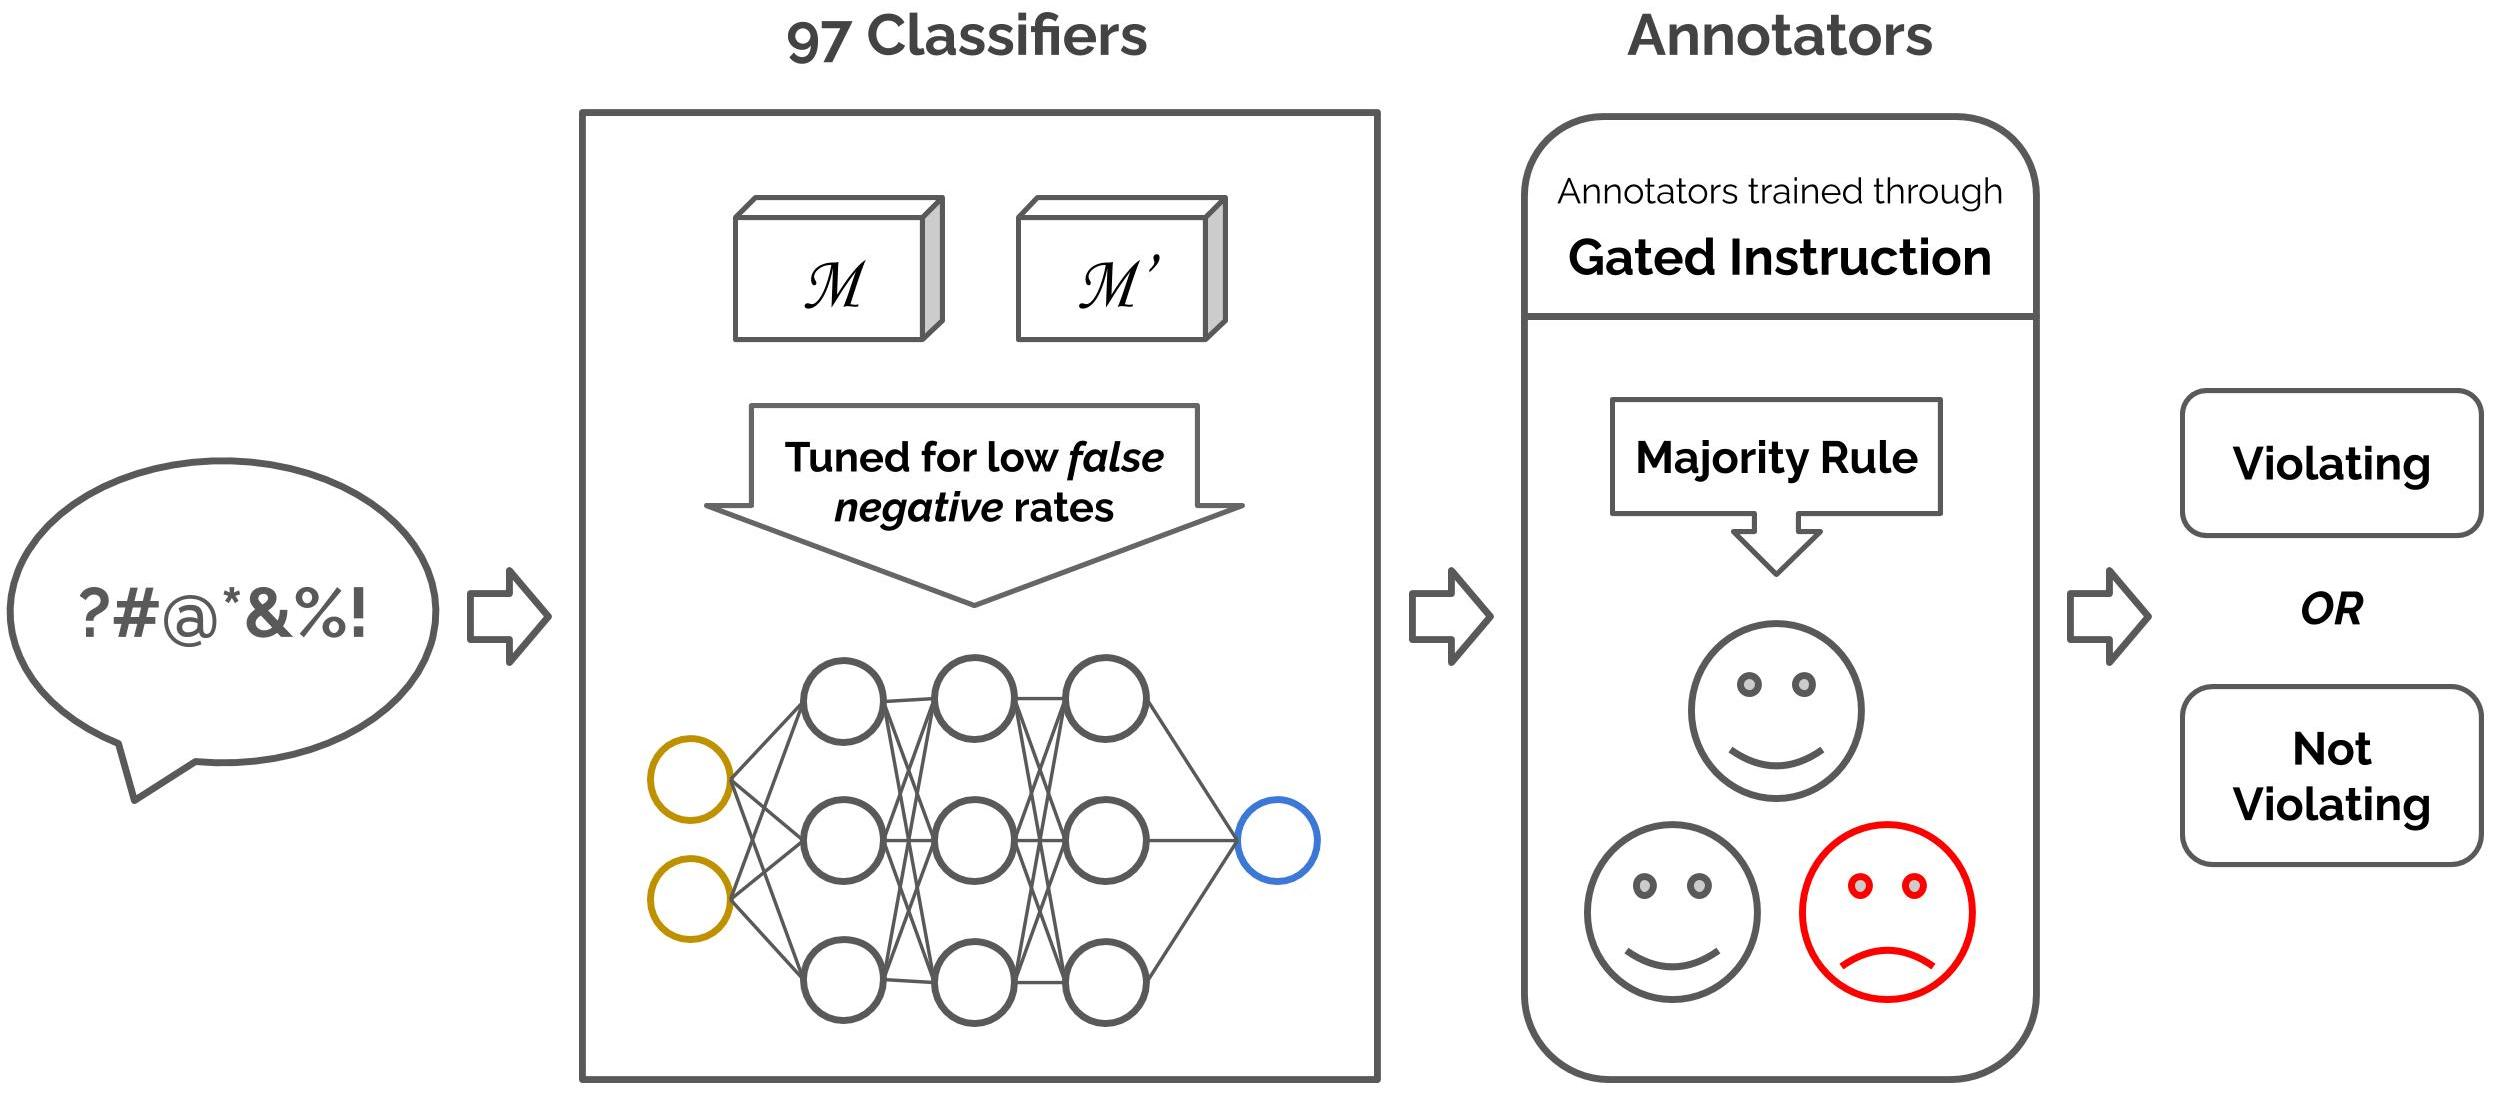
\includegraphics[width=0.90\textwidth]{content_minor_revision__Apr2022/images/Final_pipeline.jpg}
  \caption{An illustration of the human-AI pipeline for identifying violating comments. Our pipeline includes 97 subreddit classifiers that are trained using a balanced dataset of moderated and unmoderated comments, and human annotators who are trained through gated instruction~\cite{25_Liu}. Our classifiers (tuned for high recall) nominate potentially violating comments and human annotators make the final determination.}
  \Description{Human-AI pipeline}
\end{figure}




\subsection{Building the Classifiers}
Using $\mathcal{M}$ and $\mathcal{M'}$, we built 97 neural network binary classifiers, each of which was trained on the data from one of the 97 study subreddits to classify whether a given comment would be moderated on that subreddit. These classifiers collectively determine whether a comment is likely to have violated one of the macro norms and thus would have been removed on most of the subreddits. We refer to these classifiers as subreddit classifiers. 

\subsubsection{Preprocessing the data} 
We first preprocessed our dataset by putting all characters in lowercase and removing non-alphabetical characters. We then segmented our dataset into a \textit{training} dataset (70\% of all data) and \textit{testing} and \textit{validation} datasets (15\% of all data each), each with an equal number of moderated and unmoderated comments. For every study subreddits, we then used our training dataset to train word embeddings from scratch and encoded comments as fixed-length vectors, trancating and padding as needed. 

\subsubsection{Building the classifiers} 
We built our classifiers using Google's \textit{TensorFlow} and trained and validated them with the encoded dataset. The classifiers have a four-layer neural network architecture, starting with an embedding layer that takes the encoded list of integers and finds an embedding vector for each word, which we learned as we trained our network. We then pass through an average pooling layer that returns a fixed-length output vector and then through a dense layer with Rectified Linear Unit (ReLU) activation function \cite{26_TensorFlow}. Finally, we employ another dense layer with a sigmoid activation function that transforms the final output of the network into a value between 0.0 and 1.0. For our binary classification task, we identify a comment as one that would have been removed in a given subreddit if the final output of the network is greater than or equal to 0.5. 

We then fine-tuned the following four parameters for each of our subreddit classifiers using grid search where we try out exhaustive combinations of hyperparameters given candidate values:  the size of the word index used in the encoding, the length of the input vector, the number of epochs during the training phase, and the number of nodes for the ReLU layer of the neural network. These are summarized in Table 2. We optimized for the F1 score (\textit{f}-measure) on our validation dataset, achieving an average of 72.3 (std=4.32) across the 97 classifiers. This is comparable to the classifiers presented in prior work that were trained on a similar dataset \cite{4_Chancellor, chandrasekharan2019crossmod}.


% \usepackage{booktabs}


% \usepackage{booktabs}


\begin{table}[tb]
\centering
\caption{Parameters and the values used for them to fine-tune the classifiers}
\begin{tabular}{ll}
\multicolumn{1}{c}{\textbf{DESCRIPTION} } & \multicolumn{1}{c}{\textbf{SET OF VALUES} }  \\ 
\toprule
Size of the word index                    & {[}10000, 44000]                             \\
Max length of the input                   & {[}256, 512]                                 \\
Number of epochs during the training      & {[}30, 40, 50]                               \\
\# of nodes for the ReLU layer            & {[}16, 32]                                   \\
\bottomrule
\end{tabular}
\end{table}

% \begin{table}
% \centering
% \caption{Parameters and the values used for them to fine-tune the classifiers}
% \begin{tabular}{lll}
% \multicolumn{1}{c}{\textbf{PARAMETERS}} & \multicolumn{1}{c}{\textbf{DESCRIPTION}} & \multicolumn{1}{c}{\textbf{SET OF VALUES}}  \\ 
% \toprule
% \textit{$\mathcal{WI}$}                             & Size of the word index                   & {[}10000, 44000]                            \\
% \textit{$\mathcal{ML}$}                             & Max length of the input                  & {[}256, 512]                                \\
% Epochs                                  & Number of epochs during the training     & {[}30, 40, 50]                              \\
% \textit{$\mathcal{DN}$}                             & \# of nodes for the ReLU layer           & {[}16, 32]                                  \\
% \bottomrule
% \end{tabular}
% \end{table}


\subsection{Machine Learning Flags Comments}
We marked a comment as \textit{flagged} (potentially norm violating) if the number of subreddit classifiers that flagged the comment, which we call the \textit{classifier agreement score}, was greater than or equal to 80 out of 97. This threshold was selected to achieve a high recall on the ensemble classifier even at the cost of producing false positives as our pipeline includes human annotators who validate the classifier flagged comments. In other words, we wanted our process to miss as few violating comments as possible, so we deliberately used a low threshold of 80 out of 97 and passed these comments to a human review stage. This approach provides statistical power even within a realistic budget for manually annotating comments, because it results in roughly one in five flagged comments later being coded as a violation while maintaining a near-zero false negative rate.

We confirmed that this threshold indeed captures most of the violating comments: the first author manually annotated a random sample of 1,000 comments in the validation dataset from 2016 to 2017 period. This sample contained 400 comments with $< 80$ subreddit classifier agreement, 200 with $80 \leq \text{agreement} < 85 $, 200 with $85 \leq \text{agreement} < 90$, and 200 with $\geq 90$ agreement. We find that only one percent of the comments with $< 80$ classifier agreement violated at least one of the macro norms when manually inspected, whereas this number significantly increased in the subsequent sample groups (9.5\%, 12\%, and 28\% in the order of increasing classifier agreement). This low false negative rate when using a low enough agreement threshold matches the observations in a prior work that took a similar approach to classifying violating comments on Reddit \cite{chandrasekharan2019crossmod}.

In addition, to confirm that our classifier's low false negative rate holds for the comments from 2020 period, we further annotate 400 comments with classifier agreement score of less than 80 from this period randomly sampled across the study subreddits. We find our result to replicate, with roughly the same rate of 1.25\% of the sample to violate one of the macro norms. Although our subreddit classifiers were trained on comments from a 2016 to 2017 period, this low false negative rate for the comments from 2020 suggests that when combined with our human annotators, our overall pipeline still remains robust even for the newer comments. Finally, as we describe in the following section on our bootstrap sampling methods, these false negative rates are accounted for in our calculation of the confidence interval of our estimations.


\subsection{Human Annotation Validates the Flagged Comments}
\label{sec:annotation}
The tradeoff for tuning our classifiers for very few false negatives is that they produce more false positives. So we recruited human annotators to verify that the classifier flagged comments are indeed violating by asking them to code a subset of the flagged comments to see which macro norms they violate, where the subset was a random sample of the flagged comments with an even distribution across the 97 study subreddits. The definitions of these macro norms that we presented to our annotators were inspired by prior work~\cite{Chandrasekharan2018internet}, but based on our qualitative annotation discussed above, we found it appropriate to expand the definitions for some of them to better fit our data. We updated the norm described as ``opposing political views around Donald Trump'' to ``inflammatory political claims'' that covers inflammatory comments that are against the right-leaning and the left-leaning political ideologies and updated the norm described as ``hate speech that is racist or homophobic'' to ``bigotry'' that covers hate speech directed at ethnic or religious groups as well. 


\begin{figure}[tb]
  \centering
  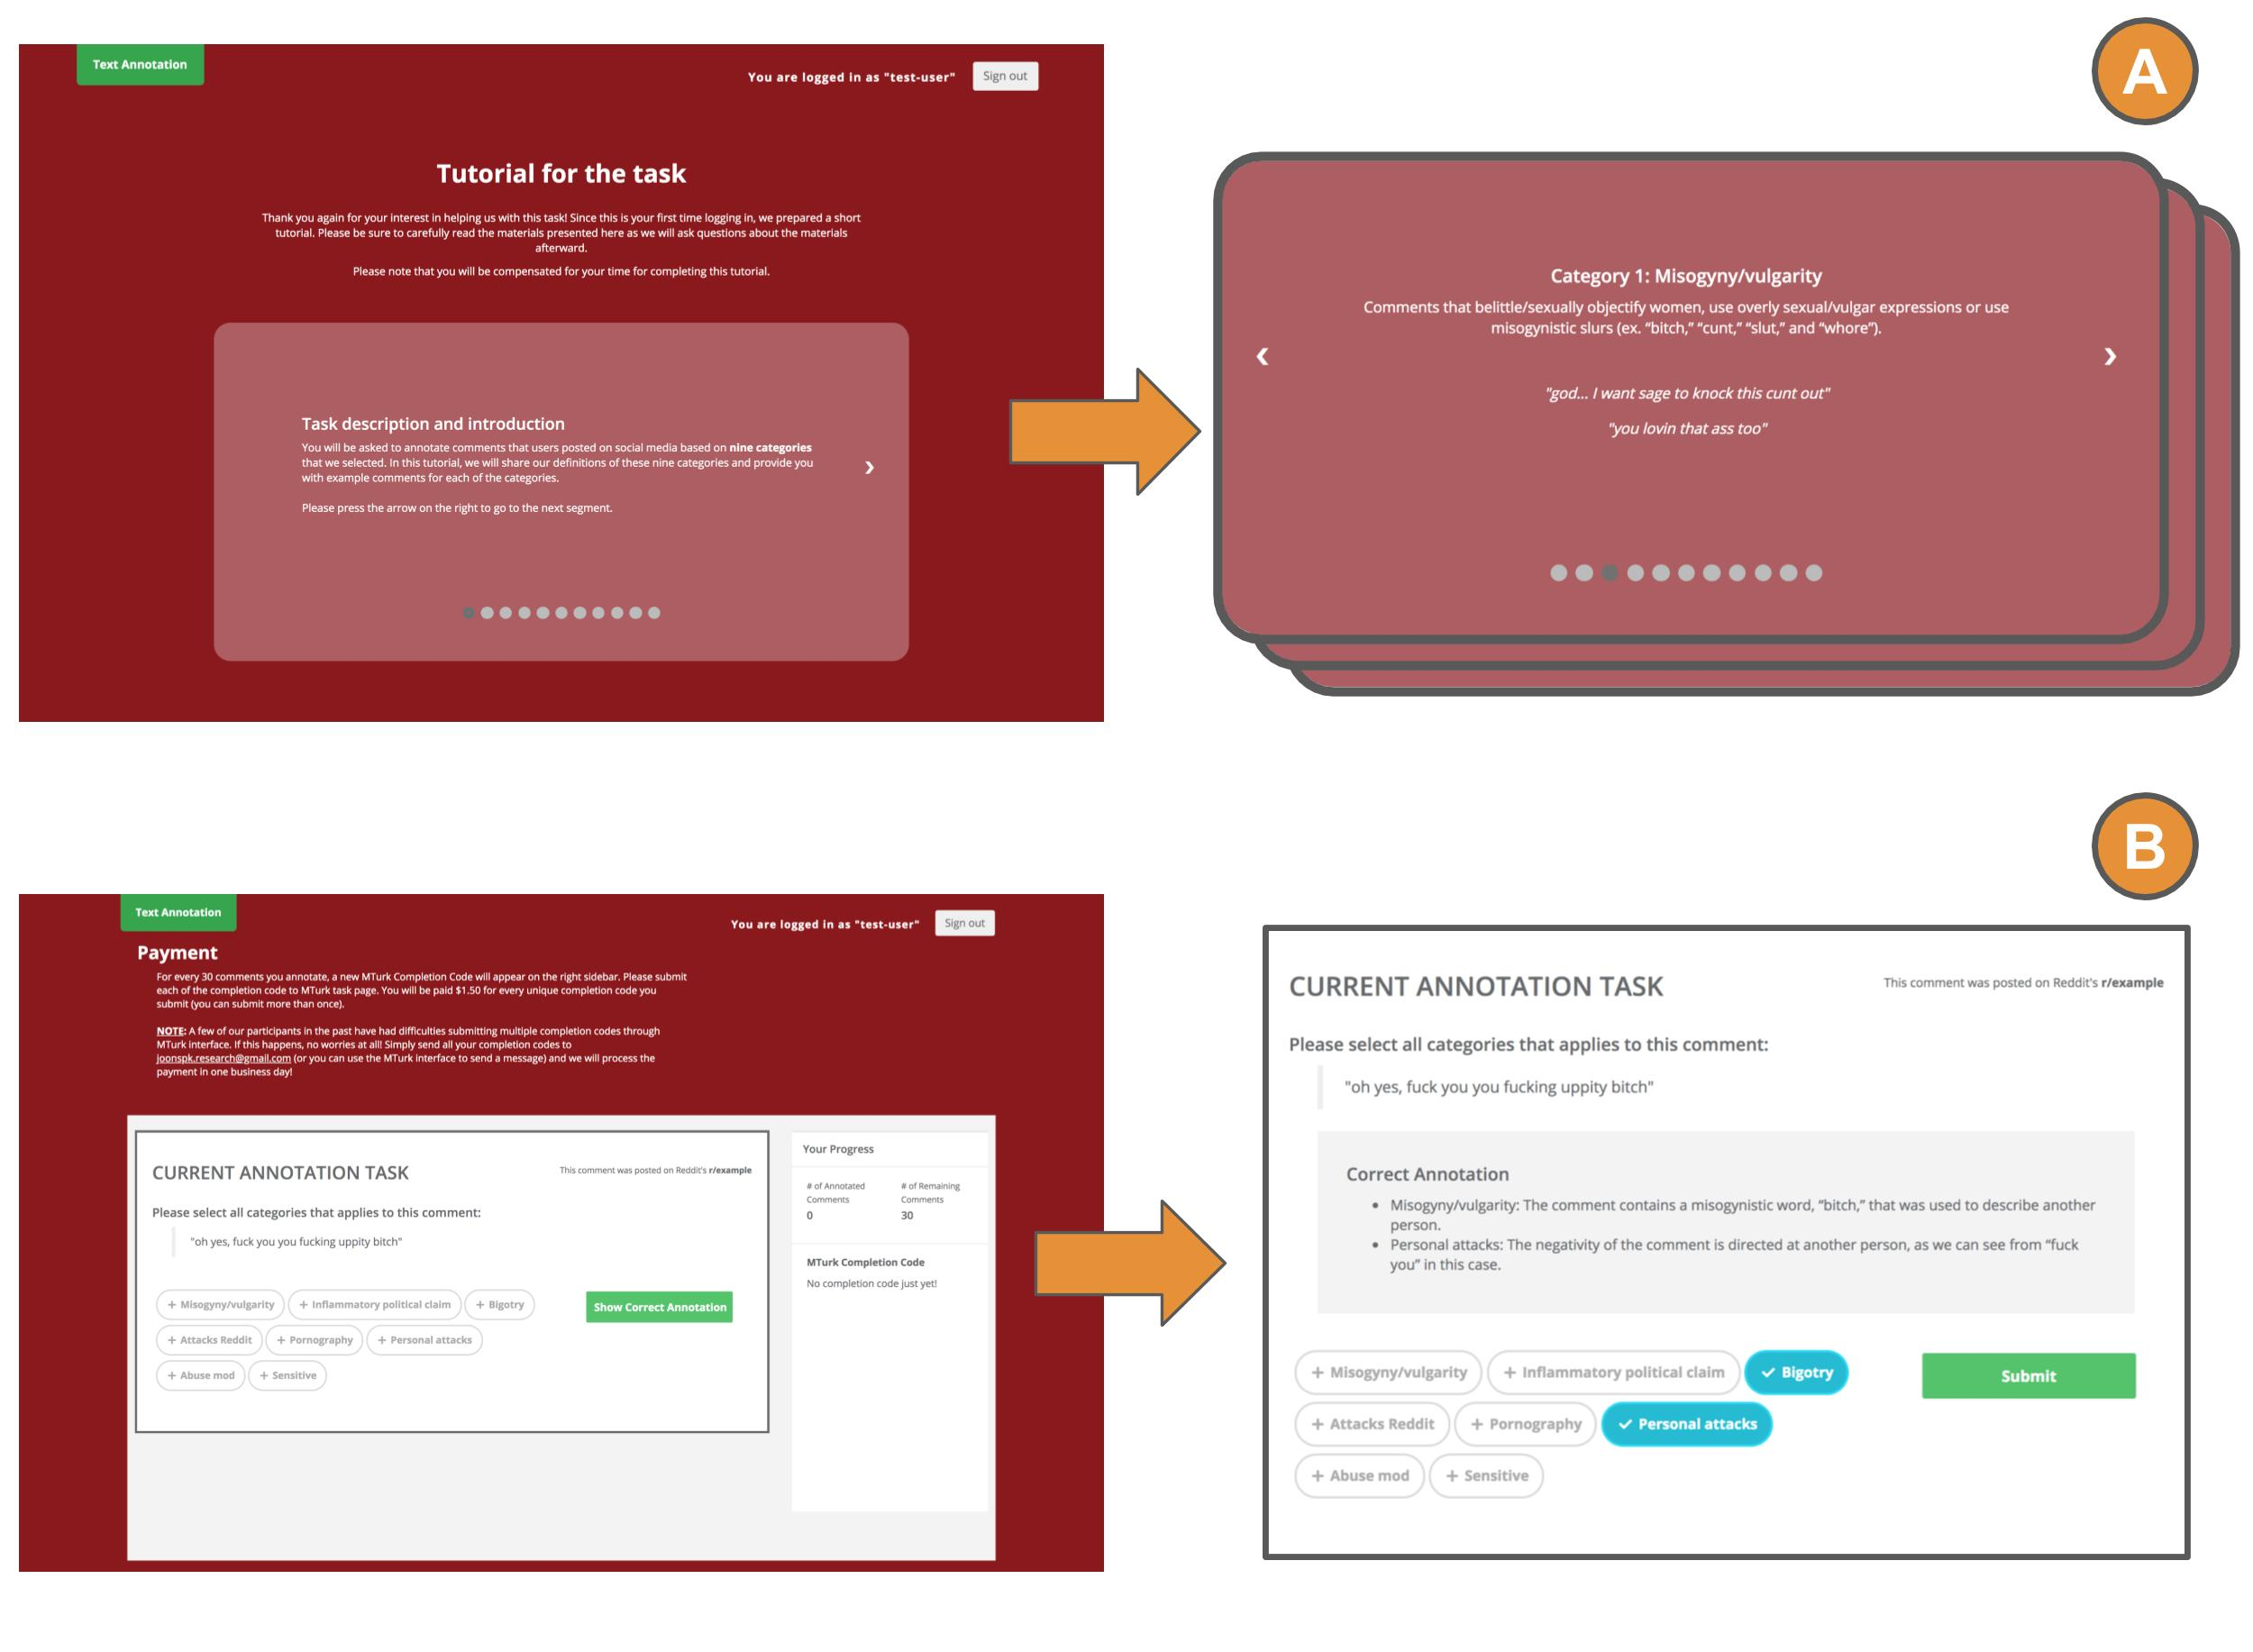
\includegraphics[width=0.98\textwidth]{content_minor_revision__Apr2022/images/annotation_interface.jpg}
  \caption{\textbf{A:} The interface for introducing the task description and eight macro norms to a new annotator. The definitions for each norms are shown one by one, accompanied by gold-standard examples that violate the norm. \textbf{B:} The interface for training and testing new annotators. Once the new annotators select their annotation, the correct annotation is shown accompanied by gold-standard examples. The interface for the main annotation task is the same but without presenting the correct annotation portion.}
  \Description{Annotation Interface}
\end{figure}



\subsubsection{Recruiting  crowd workers} 
The crowd workers were recruited from Amazon Mechanical Turk (MTurk), and they had to be at least 18 years old, living in the US, and have completed more than 1,000 Human Intelligence Tasks (HITs – MTurk’s task unit) with the minimum HIT approval rating of 98\%. In our pilot annotation task that we will describe in a subsequent subsection, our annotators took around 10 seconds (median=9.66 seconds; 75th percentile=16.99 seconds) to annotate a single comment. Based on this, we decided to pay our workers \$1.50 for every 30 comments they annotated to ensure that we are paying the majority of our workers at the rate of at least \$15.00 per hour. We decided on this rate informed by Rolf's \textit{The Fight For Fifteen} \cite{20_Rolf}.

\subsubsection{Human annotation workflow} 
Applying human annotation for non-trivial classification tasks could suffer from inaccurate annotations due accidental errors~\cite{22_Angeli, 23_Pershina, 24_Zhang}. Therefore, we designed a training and a testing phase that are inspired by the \textit{gated instruction} workflow~\cite{25_Liu} as follows to ensure that our annotators clearly understand and are proficient at the task:

Our annotators were directed to a custom-built web platform to which they could sign in with their MTurk ID. For those joining for the first time, they were redirected to the first portion of the training phase in which they were presented with 1) an overview description of the task and its goal, 2) a content warning notifying them that some comments in the task might include offensive language, and 3) the eight macro norms accompanied by their definitions and two gold-standard example comments that we manually chose from the test dataset (Figure 2-A). When they finished reviewing this content, they were asked to practice annotating 30 hand-selected, gold-standard examples of the macro norm violations handpicked from our test dataset. This was done on the actual interface used for the main annotation task that showed a comment to be annotated, and multi-select HTML form for submitting macro norm violations (Figure 2-B). The annotators could select any number of macro norms they thought the given comment violated. Importantly, during this training phase, the workers were presented with the correct annotation and explanation after each time they submitted their annotations for a given comment. Note also that, in order to avoid biasing their decisions by imposing an ``expert'' AI opinion, the workers were not told that the comments were flagged by an algorithm as potentially norm violating \cite{seering2020reconsidering}.

Of the 30 practice comments, the last 10 were effectively the test annotations; we measured our annotators’ Cronbach's alpha reliability score when compared to our gold-standard annotations, and only admitted those whose reliability score was greater than or equal to 0.7 for the last 10 training annotations. All annotators who participated in the training and testing phase were provided with a completion code they could submit to MTurk and were paid \$1.50 for their time. Those who were admitted were allowed to start the main annotation task. They could annotate as many comments as they wanted as long as there were more comments to be annotated, and were provided with a completion code they could submit to receive \$1.50 for every 30 comments they annotated. Each of the comments was seen by three unique annotators to test for majority agreement. 

During the course of this study, we recruited a total of 31 annotators who collectively annotated a total of 4,850 comments. \mrev{Finally, we followed best practices for accounting for annotator well-being during their task. In addition to presenting the aforementioned content warning, we made sure that our annotators could freely leave the study at any time if they felt uncomfortable with the annotation task. We purposefully designed our compensation scheme to ensure that we paid our participants in small increments instead of asking them for a long period of participation before receiving their compensation to ensure that our participants could receive the payment they deserve regardless of when they choose to leave the study.}


\subsubsection{Pilot} 
To confirm the robustness of this approach and  to determine the right level of compensation for the workers, we ran a pilot annotation task for which we recruited 20 annotators to partake in the training phase. Of the twenty, 8 annotators passed the testing phase and went on to annotate 194 randomly selected comments from the test dataset. The first author manually annotated the 194 comments that the annotators annotated during the aforementioned pilot tasks to establish baseline annotations to which annotators' work would be compared. In relation to the first author’s manual annotation, the majority-agreed annotation of the annotators yielded a Cronbach's alpha score of 0.86. 
